\documentclass[10pt,a4paper]{report}

\usepackage[utf8]{inputenc}
\usepackage[french]{babel}
\usepackage[T1]{fontenc}
\usepackage{amsmath}
\usepackage{amsfonts}
\usepackage{amssymb}
\usepackage{graphicx}
\usepackage{lmodern}
\usepackage{hyperref}
\usepackage{url}
\usepackage{xspace}
\usepackage{tikz}
\usepackage{listings}
%\usepackage{feynmp}
%\usepackage{tikz-feynman}

\usepackage[left=2cm,right=2cm,top=2cm,bottom=2cm]{geometry}

% biblio
%\usepackage{biblatex}
%\addbibresource{biblio.bib}

%%%%%%%%%%%%%%%%%%%%%%%%%%%%% Page de garde %%%%%%%%%%%%%%%%%%%%%%%%%%%%%
\author{Alexia \textsc{HOCINE}}

\title{Détecteur SDHCAL pour le signal  $ e^{+} e^{-} \longrightarrow \nu \nu h $ :\\Optimisation et Adaptation de l'analyse de données\\pour le Projet FCC 
}
%Stage M2 Physique, parcours SUBA\\Université de Claude Bernard Lyon 1
\date{Juillet 2022}

%%%%%%%%%%%%%%%%%%%%%%%%%%%%% Raccourçi %%%%%%%%%%%%%%%%%%%%%%%%%%%%%

% raccourci français
\newcommand{\cad}{c'est-à-dire\xspace}
\newcommand{\qqs}{quelque soit\xspace}
\newcommand{\MS}{Modèle Standard\xspace}


% nom informatique
\newcommand{\ROOT}{\texttt{ROOT}\xspace}
\newcommand{\SLCIO}{\texttt{SLCIO}\xspace}
\newcommand{\iLCSoft}{\texttt{iLCSoft}\xspace}
\newcommand{\LCIO}{\texttt{LCIO}\xspace}
\newcommand{\Marlin}{\texttt{Marlin}\xspace}
%\newcommand{\Key4HEP}{\texttt{Key4HEP}\xspace}
\newcommand{\Gaudi}{\texttt{Gaudi}\xspace}

\newcommand{\nnhAnalysis}{\texttt{nnhAnalysis}\xspace}

\newcommand{\original}{\texttt{original}\xspace}
\newcommand{\ilcsoft}{\texttt{ilcsoft}\xspace}
\newcommand{\fcc}{\texttt{fcc}\xspace}

\newcommand{\minidstmarker}{\texttt{miniDSTMaker}\xspace}
\newcommand{\convert}{\texttt{convert}\xspace}
\newcommand{\processor}{\texttt{processor}\xspace}
\newcommand{\analysis}{\texttt{analysis}\xspace}


% nom de particules
\newcommand{\particle}[1]{$\texttt{#1}$}

\newcommand{\bbar}{\overline{b}}

\newcommand{\Wstar}{W^{\star}}

\newcommand{\electron}{e^{+}}
\newcommand{\positron}{e^{-}}

\newcommand{\nnh}{\nu \nu h}

% physique
\newcommand{\GeV}{\texttt{GeV}}
\newcommand{\TeV}{\texttt{TeV}}

% LaTeX

\newcommand{\be}{\begin{enumerate}}
\newcommand{\ee}{\end{enumerate}}

\newcommand{\bi}{\begin{itemize}}
\newcommand{\ei}{\end{itemize}}


%%%%%%%%%%%%%%%%%%%%%%%%%%%%% corps du document %%%%%%%%%%%%%%%%%%%%%%%%%%%%%

\begin{document}

% Page de Garde

\begin{titlepage}
	\begin{center}
		
    		\vspace*{3cm}

    		\LARGE
    		\textbf{Détecteur SDHCAL pour le signal  $ e^{+} e^{-} \longrightarrow \nu \nu h $ :\\Optimisation et Adaptation de l'analyse de données\\pour le Projet FCC}

    		\vspace{1.5cm}

    		Alexia \textsc{HOCINE}\\
    		\vspace{0.4cm}
    		\large 
    			Étudiante en M2 Physique SUBA à l'UCBL1
    		
		\vspace{1.5cm}
		\Large
		Supervisé par Gérald \textsc{Grenier}\\
    		\vspace{0.4cm}
    		\large 
    			Maître de Conférence - UCBL1\\
    			Enseignant-Chercheur - IP2I, CNRS, IN2P3\\
    			Membre des collaborations CALICE, CMS et ILD\\
    			Corresponsable du groupe SDHCAL au sein de la collaboration CALICE

    		\vfill

		
\includegraphics[width=5cm]{../img/Logo_IP2I.png}
 		
\includegraphics[width=5cm]{../img/UdL-logo.png}

		\vspace{3cm} 

    		Rapport de Stage - Master 2 Physique SUBA\\
    		Université de Claude Bernard Lyon 1 \\    		

    		\vspace{1.5cm}
    		
    		Avril-Juillet 2022
    
 		
	\end{center}

\end{titlepage}

%%%%%%%%%%%%%%%%%%%%%%%%%%%%%

% Préambule

\chapter*{Préambule}

\section*{Remerciements}

Je souhaite d'abord remercier Gérald \textsc{Grenier} pour m'avoir donner la chance de montrer ce que je peux faire. Et aussi pour son encadrement, son accompagnement et son temps.

Je souhaite plus largement remercier mon équipe, Gérald \textsc{Grenier}, Imad \textsc{Laktineh} et Clément \textsc{Devanne}, pour l'atmosphère positive, détendue et stimulante.

Et plus largement, les employés de l'IP2I pour leur gentillesse et leur accueil.

\section*{Participation à la \textit{Geek and Japan Touch}}

Au cours de mon stage, j'ai participé à l'atelier tenu par l'IP2I à la \textit{Geek and Japon Touch}, organisé par Stéphanie \textsc{Beauceron} (IP2I, CNRS, CMS).

Durant ce week-end, avec 2 autres chercheuses (non physiciennes), Florence \textsc{Boyer} et Liliane \textsc{De Araujo}, on a tenu un débat sur le film \textit{Don't look up : Déni Cosmique} de Adam \textsc{McKay}, sur la crédibilité du discours scientifiques.

Ensuite sur le stand, j'ai pu expliquer les bases scientifiques et des recherches menées par le CNRS et CMS, ainsi que Virgo au près du grand publique. 

De plus, j'ai aussi animé le stand de l'association ?? dont l'objectif est d'expliquer les principes de base de la gravité en 2D avec un drap tenu.

%%%%%%%%%%%%%%%%%%%%%%%%%%%%%

\tableofcontents

%%%%%%%%%%%%%%%%%%%%%%%%%%%%%
ev Introduction

\chapter{Introduction}

\section{La Physique des Collisionneurs}

Le principe des collisionneurs est simple, on accélère des particules à des 
énergies cinétiques suffisantes pour provoquer des collisions inélastiques, et ainsi comprendre les interactions fondamentales et les constituants élémentaires de la matière.\\

On distingue 2 familles de collisionneurs en fonction des particules qui sont utilisés.

\subsection{Collisionneurs hadroniques}

Les collisionneurs hadroniques utilisent des hadrons, qui sont des 
particules complexes composées de 3 quarks et de gluons\footnote{Gluon : boson médiateur de l'interaction forte qui maintiennent les quarks ensembles.}. 
Par exemple au LHC\footnote{LHC : Large Hadron Collider, CERN}, on utilise des protons, composés de 2 quarks up et d'1 quark down. 

Comme il s'agit de particules composites, ce sont pas les protons qui collisionnent directement mais ces constituants, appelés partons. 
Chacun porte une fraction indéterminée de l'énergie du proton. 
On ignore donc l'énergie de la collision en amont, il s'agit d'un paramètre libre. 

C'est pourquoi, ils sont utiles pour la découverte de nouvelles particules de masse inconnue, puisqu'ils permettent de balayer tout le spectre de masse sous la gamme d'énergie du collisionneur (au LHC < 14 $\TeV$)\footnote{D'où l'intérêt de nouveaux collisionneurs à des énergies plus élevées et donc des masses de particules produites plus lourdes.}.

\subsection{Collisionneurs leptoniques}

En revanche, les collisionneurs leptoniques utilisent des leptons, qui sont des particules élémentaires. 
Comme le LEP\footnote{LEP : Large Electron-Positron, le prédécesseur du LHC, même tunnel}, qui collisionnait des électrons et des positrons \cite{cern:lep}.

Cette fois-ci, chaque lepton qui collisionne, possède une énergie complète donc connue. 
Puisqu'on leur impulse une énergie précise, ainsi on augmente la statistique pour un certain niveau d'énergie.
Ces collisionneurs sont donc utilisés pour la recherche de précision.\\

Les prochaines générations de collisionneurs, comme ILC, CEPC, CLIC et FCC, ce sont des collisionneurs leptoniques. 
Leur objectif est de préciser les données déjà obtenues, notamment sur le boson de Higgs découvert en 2012 par le LHC\footnote{Higgs : était la pièce manquante du modèle standard des particules, car il permet aux particules d'acquérir une masse}.

\section{Physique du boson de Higgs}

\subsection{Production du boson de Higgs}

Concrètement, on ne mesure pas directement le boson de Higgs mais ses produits de désintégrations sous la forme de jet.
Ainsi on cherche à améliorer la résolutions en énergie de ces jets que l'on détecte \cite{liu:tel-03405418}.

\subsection{Détecteur}

En physique des particules, on utilise des détecteurs appelés calorimètres pour mesurer l'énergie des particules. 
Cette énergie va être déposer par ionisation dans le matériau le long de la trajectoire des particules qui le traverse. 
Il faut donc des algorithmes de reconstruction pour déduire les énergies, les types de particules et les trajectoires.

Pour cela, on utilise des calorimètres à grande granularité qui permet une très bonne performance des Algorithmes de Flux de Particules (PFA) \cite{liu:tel-03405418}. \\

C'est dans ce cadre que la collaboration internationale CALICE, à développer le premier prototype de la famille de calorimètre granulaire SDHCAL, pour Semi-Digital Hadronic CALorimeter, qui a été développé en grande partie à l'IP2I dans l'équipe CMS, auquel j'appartiens pour ce stage.

\subsection{Collisions}

Au cours, de ce stage, je me suis concentrée sur les collisions de type \texttt{nnh} pour neutrino-neutrino-higgs.

Dont voici les diagrammes de Feynman :

\begin{figure}[h!]
	\centering
	\begin{tikzpicture}
	
	\end{tikzpicture}
	\caption{Diagramme de Feynmann de collision $ e^{+} e^{-} \longrightarrow \nu \nu h $}
	\label{Feynman}
\end{figure}

\section{Présentation \& Objectif du Stage}

Pour ce stage, j'ai récupéré les codes de Guillaume \textsc{Garillot}, qui les a développé en 2021 au cours de son post-doctorat à l'IP2I. 
Ils sont en libre accès à l'adresse \url{https://github.com/ggarillot/nnhAnalysis/tree/refactor}.\\

Ce programme \nnhAnalysis permet l'étude de fichiers \SLCIO pour la collision :
\begin{equation}
	\positron \electron \longrightarrow \nnh
\end{equation}

Et l'analyse des canaux de désintégration :

\begin{align}
	h &\longrightarrow W \Wstar \longrightarrow qqqq \\
	h &\longrightarrow b \bbar 
\end{align}

Pour cela, il a utilisé les suites logiciels de \iLCSoft, \url{https://github.com/iLCSoft} (plus précisément \LCIO et \Marlin), qui sont les anciennes suites logicielles.
Mais les nouveaux projets de collisionneurs utiliseront \texttt{Key4HEP} et \Gaudi.\\

Mon objectif est double. Dans un premier temps, comprendre et optimiser les codes existants, \cad le programme \nnhAnalysis de Guillaume \textsc{Garillot} qui utilise \LCIO, \Marlin. 
Puis, je vais transformer son programme pour qu'il puisque correspondre aux nouvelles normes des collisionneurs leptoniques, \texttt{Key4HEP} et \Gaudi.

%\feynmandiagram [horizontal=a to b] {
%  i1 -- [fermion] a -- [fermion] i2,
%  a -- [photon] b,
%  f1 -- [fermion] b -- [fermion] f2,
%};



%%%%%%%%%%%%%%%%%%%%%%%%%%%%%

\chapter{\texttt{ILC}}

\section{Présentation du Projet ILC}

Le projet ILC (International Linear Collider) est un collisionneur linéaire, électron-positron, de 31 km conçu pour atteindre une énergie de centre de masse de 500 \GeV \cite{cern:ilc}. \\

\begin{figure}[h!]
	\center
	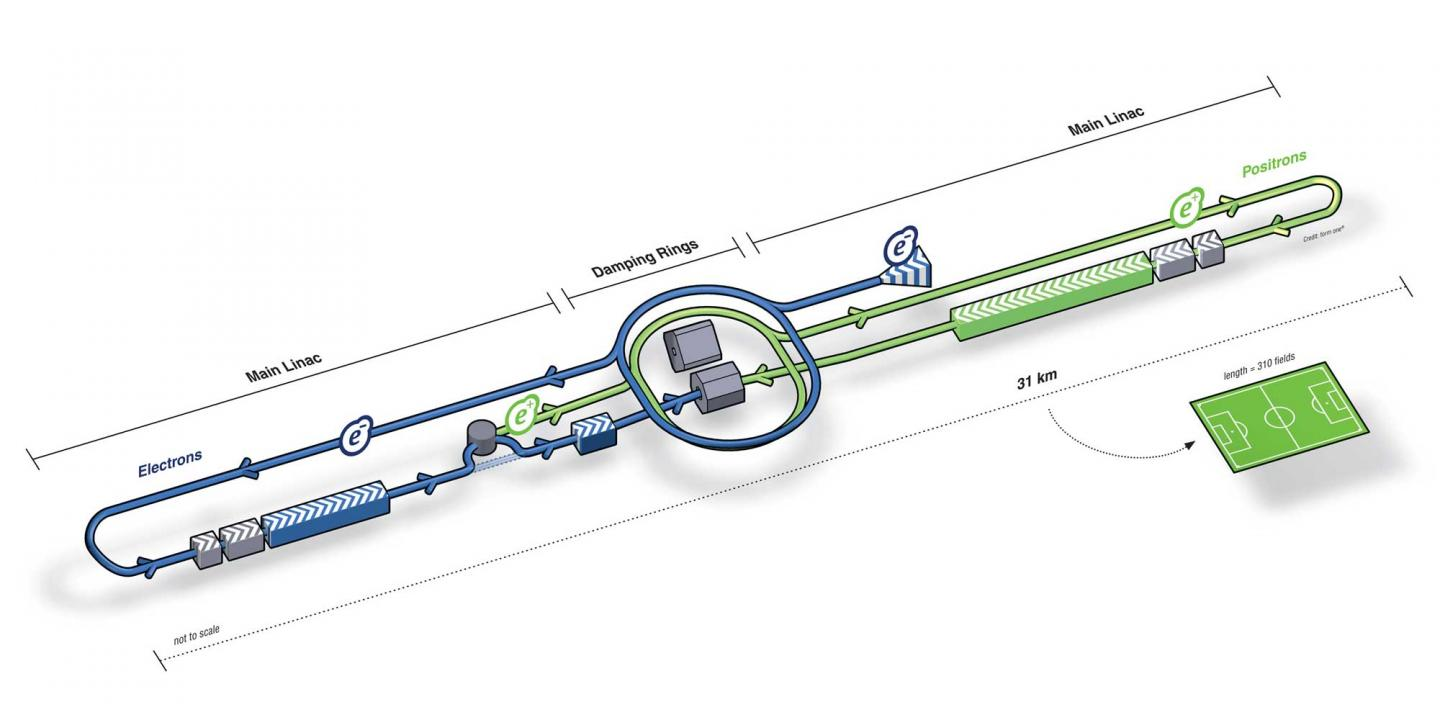
\includegraphics[width=\textwidth]{../img/ilc.jpg} 
	\caption{Schéma ILC\cite{cern:ilc}}
	\label{ilc:schema}
\end{figure}

L'objectif de l'ILC est de produire beaucoup de boson de Higgs notamment pour découvrir s'il y en a d'autre génération du boson de Higgs. Et plus globalement pour rechercher de la nouvelle physique, par de nouveaux écarts avec le \MS.\\

Ce projet est toujours en attente pour commencer sa construction, probablement dans les montagne du Nord du Japon. Et le détecteur SDHCAL est en course pour y être installer. C'est pourquoi, l'IP2I développe des programme d'analyse en parallèle de ce détecteur.

\section{Projet numérique : \original}

% Contexte
Pour ce stage j'ai récupéré les codes de Guillaume Garillot, qui les a développé en 2021 au cours de son post-doctorat à l'IP2I. 

Son programme permet l'identification et l'analyse statistique de collision du détecteur SDHCAL.

\subsection{Données initiales}

% données distantes : miniDSTMarker
La première étape est de récupérer les données (aujourd'hui simulées, plus tard obtenues dans le détecteur) sur le serveur distant où elles sont stockées, grâce au programme \minidstmarker. 

Mais pour le temps du stage je n'ai pas obtenu l'accès à ce serveur donc je n'ai pas pu utilisé cette partie de code. Je l'ai donc pas réutilisé dans ma propre version.\\

% données locales
Initialement, on m'a mis à disposition certains de ces fichiers \SLCIO, ceux des collisions de 250 \GeV. 
Chaque fichier est rangés dans un des 66 dossiers (Figure~\ref{listeProcessus}), qui correspond au code du type de processus.

\begin{figure}[h!]
	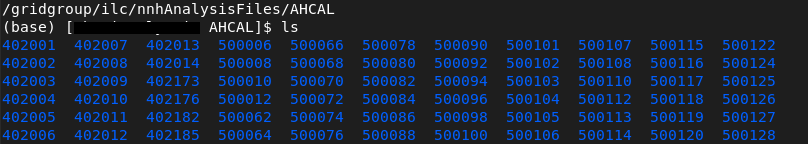
\includegraphics[width=\textwidth]{../img/listeProcessus.png} 
	\caption{Les noms des dossiers qui correspondent aux numéros de processus}
	\label{listeProcessus}
\end{figure}

Ce dossier a été placé sur le serveur local de l'IP2I : \texttt{/gridgroup/ilc/nnhAnalysisFiles/AHCAL}.

%\paragraph{Numéro des processus ???}

\subsection{Conversion des fichiers initiaux en fichiers \ROOT}

Grâce au programme \processor on va pouvoir convertir les fichiers initiaux \SLCIO en fichiers \ROOT standards, afin de pouvoir les analyser.\\

On obtient ainsi pour chaque dossier de fichier de donnée \SLCIO un fichier \ROOT en sortie, \cad que l'on obtiendra un arbre \ROOT par type de processus.\\

Ce programme doit être robuste et donc à partir des mêmes fichiers toujours générer les fichiers \ROOT strictement identiques.

\subsection{Analyses des collisions}

Avant de commencer l'analyse des fichiers \ROOT générés précédemment, on va terminer ce que le programme \processor avait commencé, et fusionner l'intégralité de ces fichiers en un seul gros fichier \texttt{DATA.root}, grâce à la commande \texttt{hadd}. 
Cette commande a été développé par le CERN et elle fusionne tous les histogrammes de différents fichiers en un seul. 

Donc là aussi tous les fichiers \texttt{DATA.root} doivent être strictement identique. \\

Pour la deuxième étape de ce programme \analysis on va de nouveau séparer nos données en 4 fichiers distincts. 
Mais au lieu de les séparer par leur numéro de processus, qui est un critère numérique, on va les diviser par le type de particules produit par le boson de Higgs, soit $b\bbar$, soit $W\Wstar$, et par la polarisation de particules incidentes, \cad l'électron et le positron avec une polarisation de -0,8 et 0,3 soit nulles.
Ce qui va nous créer les 4 fichiers suivants :

\begin{figure}[h!]
	\centering
	\begin{lstlisting}
			split_bb_e-0.8_p+0.3.root
			split_bb_e+0_p+0.root
			split_ww_e-0.8_p+0.3.root
			split_ww_e+0_p+0.root
	\end{lstlisting}
	\label{files:split}
	\caption{Fichiers où les évènements sont séparés en fonction des caractéristiques des polarisations des particules incidentes et des types de particules résultantes.}
\end{figure}

Pour trier les données du fichier \texttt{DATA.root}, on va utiliser des arbres de décision, BDT pour Boosted Decision Tree. 


HERE !!!!!!!!!!!!!!!


Une fois encore l'API du CERN, nous aura été très utile. Mais cette fois-ci les fichiers créés sont équivalents mais pas identique. Car les BDT utilisent la génération aléatoire, ce qui engendre des variations dans les entraînements.\\

Pour terminer, on peut effectuer l'analyse à proprement parlé de nos données.


HERE !!!!!!!!!!!!!!!


Et même si cette analyse sera toujours la même \qqs les fichiers \texttt{split\_XX.root}, c'est dernier étant légèrement différent d'un entraînement à l'autre les résultats statistiques seront, là encore, légèrement différent mais équivalent.

\section{Projet numérique \ilcsoft}

\subsection{Données}
Initialement, on m'a mis à disposition des fichiers \SLCIO, qui sera le format de fichier du détecteur.
Chaque fichier est rangés dans un des 66 dossiers (Figure~\ref{listeProcessus}), qui correspond au code du type de processus.

\begin{figure}[h!]
	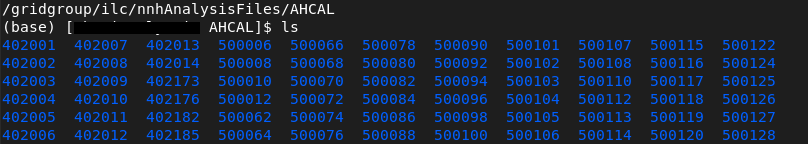
\includegraphics[width=\textwidth]{../img/listeProcessus.png} 
	\caption{Les noms des dossiers qui correspondent aux numéros de processus}
	\label{listeProcessus}
\end{figure}

%\paragraph{Numéro des processus ???}

\subsection{Programme : \processor}

\subsubsection{Méthodes}

On cherche à convertir ces fichiers \SLCIO en arbre \ROOT par processus.

\subsubsection{Résultats}

%\paragraph{Des fichiers \ROOT :}
Chaque dossier de fichier de donnée \SLCIO produira un fichier \ROOT en sortie, \cad que l'on obtiendra un arbre \ROOT par processus.


\subsubsection{Interprétation}

\subsection{Programme \analysis}

\subsubsection{Données}

On récupère les fichiers \ROOT du programme \processor précédent. 

$ hadd $ qui va créer le fichier DATA.root

\subsubsection{Méthodes}

\paragraph{\texttt{BDT}}

Entrainement

\paragraph{L'analyse}


\subsubsection{Résultats}

\paragraph{Vérification des résultats}
Comparaison entre les différents séries d'analyse, basée sur les même fichiers \ROOT, mais un autre entraînement de BDT.

\subsubsection{Interprétation}

%%%%%%%%%%%%%%%%%%%%%%%%%%%%%

\chapter{\texttt{FCC}}

\section{Projet FCC}

\subsection{Présentation}

Le FCC (Futur Collisionneur Circulaire) est le projet du CERN pour remplacer 
leur collisionneur actuelle, le LHC (Large Hadronic Collider). 
Dont la fin de l'exploitation est prévu en 2040 \cite{cern:fcc}

Pour le FCC, on prévoit un anneau de 100 km, contre 27 km pour le LEP et le LHC 
(comme montrer Figure~\ref{fcc:img}).
Ce qui devrait nous permettra d'atteindre une énergie de 100 \TeV contre 13 \TeV
actuellement pour le LHC.

L'objectif est de rechercher d'une nouvelle physique, en mettant au jour de 
déviation avec le modèle standard.


\begin{figure}[h!]
    \centering
    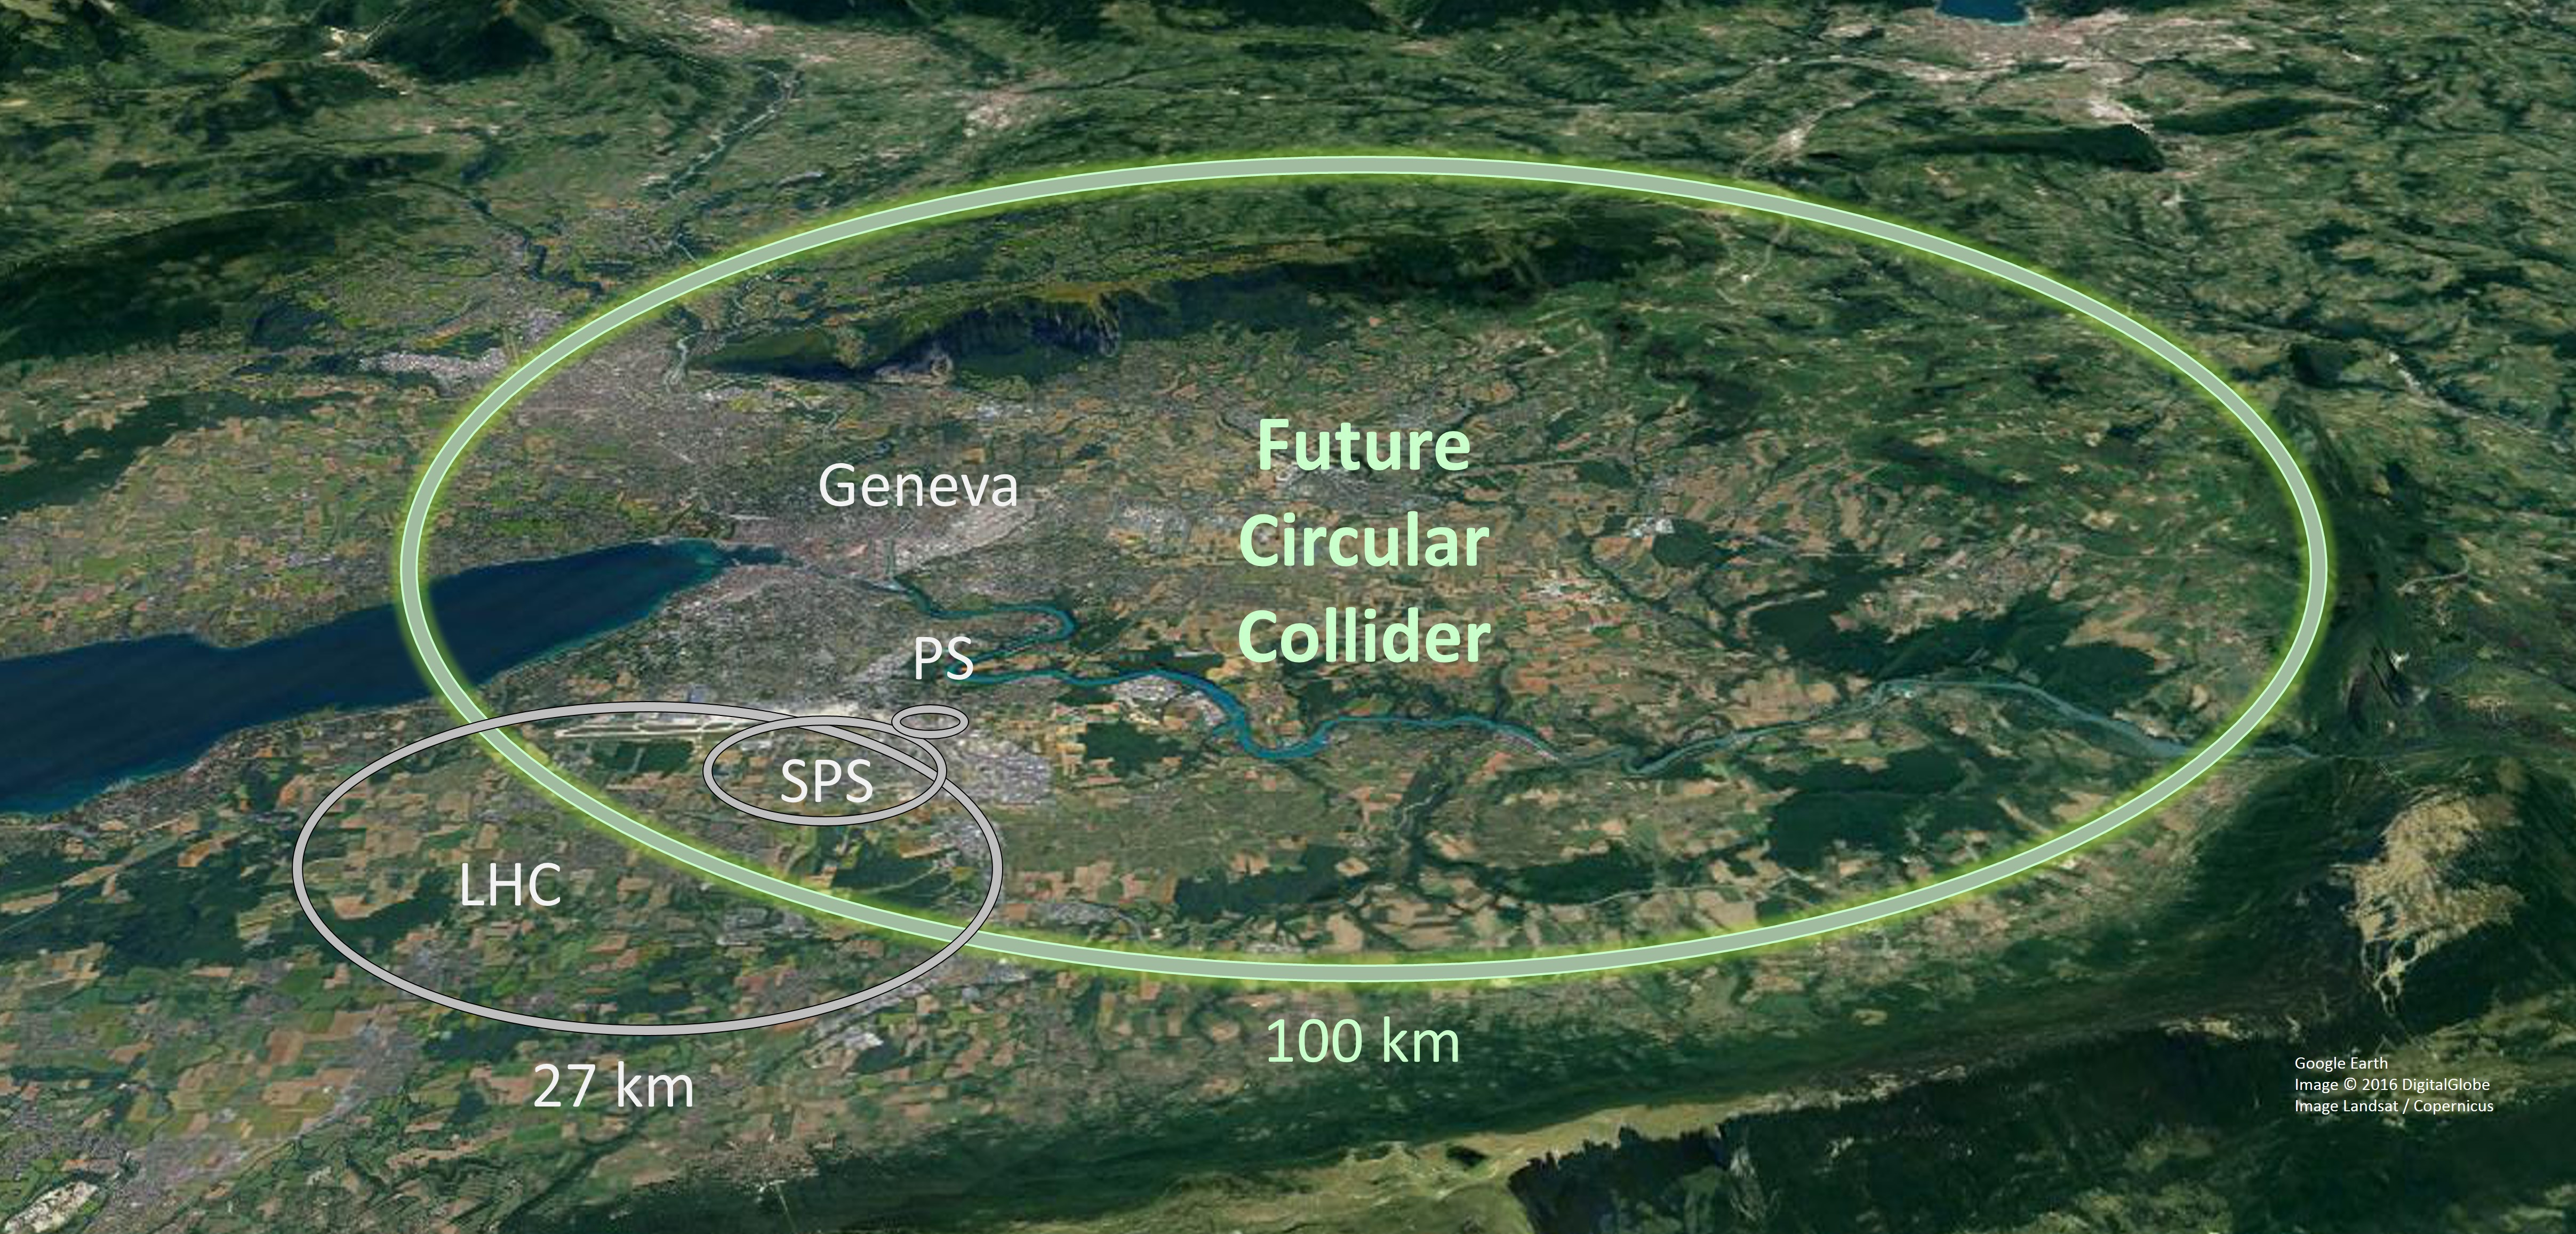
\includegraphics[width=\textwidth]{../img/FCC.jpg}
    \caption{https://cds.cern.ch/images/OPEN-PHO-ACCEL-2019-001-2}
    \label{fcc:img}
\end{figure}

\section{Développement Numérique}

Mon objectif dans ce stage est de transformer les codes développés par Guillaume 
\textsc{Garillot} lors de son post-doctorat pour le projet ILC pour ce projet 
qui n'utilise pas les mêmes suites logiciels.

\texttt{Gaudi}

\texttt{EDM4hep}

\section{Travail de Stage}

\section{Comparaison avec \texttt{iLCSoft}}

%%%%%%%%%%%%%%%%%%%%%%%%%%%%%

\chapter{Outils Numériques}

\section{\texttt{nnhScript}}
\url{https://github.com/alexhxia/nnhAnalysis/tree/main/nnhScript}

\section{\texttt{nnhTest}}

Pour tester les programmes générer avec \texttt{nnhProgram}, j'ai développé 4 programmes en \texttt{python} : 

\begin{figure}[h!]
	\center
	\begin{tabular}{| c | c | c |}
		\hline
			\texttt{•} & \texttt{Processus} & \texttt{Analysis} \\
		\hline
			\texttt{Completed} & \texttt{testProcessorCompleted.py} & \texttt{testAnalysisCompleted.py} \\
		\hline
			\texttt{Same} & \texttt{testProcessorSame.py} & \texttt{testAnalysisSame.py} \\
		\hline
	\end{tabular}
	\caption{Tableau récapitulatif des fonctions de tests}
\end{figure}

\subsection{Programmes \texttt{testXxCompleted.py}}

L'objectif de ce type de programme est de tester si tous les fichiers ont été généré.

\subsubsection{Programmes \texttt{testProcessorCompleted.py}}

Le processus est complet si tous les dossiers de 

\subsubsection{Programmes \texttt{testAnalysisCompleted.py}}


\subsection{Programmes \texttt{testXxSame.py}}

\subsubsection{Programmes \texttt{testProcessorSame.py}}

\subsubsection{Programmes \texttt{testAnalysisSame.py}}



\url{https://github.com/alexhxia/nnhAnalysis/tree/main/nnhTest}

%%%%%%%%%%%%%%%%%%%%%%%%%%%%%

\chapter{Exemples de Résultats Physiques}

%%%%%%%%%%%%%%%%%%%%%%%%%%%%%
\chapter{Conclusion}


%%%%%%%%%%%%%%%%%%%%%%%%%%%%%

\begin{appendix}

%%%%%%%%%%%%%%%%%%%%%%%%%%%%%

\chapter{Résumé du travail effectué}

\section{Bibliographie}

\paragraph{\url{https://tel.archives-ouvertes.fr/tel-03405418}}
\begin{itemize}
	\item Étude du calorilmètre hadronique semi-digital et étude du canal physique 
	$$ \positron \electron \longrightarrow \nnh \ (H \longrightarrow WW \longrightarrow qqqq)$$ 
	au collisionneur circulaire électron positon (CEPC) 
	\item Bing Liu, IP2I
	\item 2020
\end{itemize}

\paragraph{\url{https://tel.archives-ouvertes.fr/tel-02141420}}
\begin{itemize}
	\item Étude des gerbes hadroniques dans un calorimètre à grande granularité et étude du canal $$ \positron \electron \longrightarrow HZ \ (Z \longrightarrow qq) $$ dans les futurs collisionneurs leptoniques
	\item Guillaume Garillot, IPNL
	\item 2019
\end{itemize}

\section{Tutoriels}

\begin{description}
	\item[\texttt{LCIO}] \url{https://github.com/iLCSoft/LCIO}
	\item[\texttt{ILDConfig}] \url{https://github.com/iLCSoft/ILDConfig}
	\item[\texttt{Marlin}] \url{https://github.com/iLCSoft/Marlin}
	\item[\texttt{key4hep}] \url{https://github.com/key4hep/k4MarlinWrapper}
\end{description}

\section{Code initial}

\url{https://github.com/ggarillot/nnhAnalysis/tree/refactor}

\section{Code final}

\url{https://github.com/alexhxia/nnhAnalysis}

%%%%%%%%%%%%%%%%%%%%%%%%%%%%%

\chapter{Organisation du Projet}

\section{Organisation initiale}

\begin{figure}[h!]
	\center
	\begin{tikzpicture}

		\tikzstyle{home}=[draw, rectangle, fill=red!50, text=black, rounded corners=3pt]		
		
		\tikzstyle{directory}=[draw, rectangle, fill=gray!30, text=black, rounded corners=3pt]

		\node[home] (A) at (0,0) {\texttt{nnhAnalysis}};
		
		\node[directory] (AM) at (-4,-2.5){\minidstmarker};
		\node[directory] (AP) at (0,-2.5) {\processor};
		\node[directory] (AA) at (4,-2.5) {\analysis};
		
		
		\tikzstyle{linkDir}=[->,dotted,very thick,>=latex]
		
		\draw[linkDir] (A)--(AM);
		\draw[linkDir] (A)--(AP); 
		\draw[linkDir] (A)--(AA);
		
	\end{tikzpicture}
	\caption{
		Organisation des dossiers de mon Projet - \url{https://github.com/ggarillot/nnhAnalysis/tree/refactor}
	}
	\label{orga:begin}
\end{figure}

\section{Organisation finale}

\begin{figure}[h!]
	\center
	\begin{tikzpicture}
	
		\tikzstyle{home}=[draw, rectangle, fill=red!50, text=black, rounded corners=3pt]		
	
		\tikzstyle{directory}=[draw, rectangle, fill=gray!30, text=black, rounded corners=3pt]

		\node[directory] (A) at (0,0) {\texttt{nnhAnalysis}};
		
		\node[directory] (S) at (-4.5,-1.5) {\texttt{nnhScript}};
		\node[directory] (P) at (-1.5,-1.5) {\texttt{nnhProgram}};
		\node[directory] (R) at ( 1.5,-1.5) {\texttt{nnhResult}};
		\node[directory] (T) at ( 4.5,-1.5) {\texttt{nnhTest}};
		
		\node[home] (O) at (-5.5,-3) {\texttt{original}};
		\node[home] (I) at (-1.5,-3) {\texttt{ilcsoft}};
		\node[home] (F) at ( 3.5,-3) {\texttt{fcc}};
		
		\node[directory] (OP) at (-7,-4.5) {\texttt{processor}};
		\node[directory] (OA) at (-5,-4.5) {\texttt{analysis}};
		
		\node[directory] (IP) at (-2.5,-4.5) {\texttt{processor}};
		\node[directory] (IA) at (-0.5,-4.5) {\texttt{analysis}};
		
		\node[directory] (FC) at (1.5,-4.5) {\texttt{convert}};
		\node[directory] (FP) at (3.5,-4.5) {\texttt{processor}};
		\node[directory] (FA) at (5.5,-4.5) {\texttt{analysis}};
		
		
%		\tikzstyle{files}=[rectangle, draw, fill=red!40, text=black, below right]		
%		
%		\node[files] (r) at (-2.2,-2) {
%				\texttt{...}
%		};
%		\node[files, text width=3cm] (s) at (0.7,-2) {
%				\texttt{nnh.sh}
%				\texttt{nnhProcessor.sh}
%				\texttt{nnhAnalysis.sh}
%				\texttt{prepaeBDT.sh}
%				\texttt{launchBDT.sh}
%				\texttt{nnhExport.sh}
%		};
%		\node[files, text width=5cm] (t) at (4.3,-2) {
%				\texttt{testProcessorCompleted.py}
%				\texttt{testProcessorSame.py}
%				\texttt{testAnalysisCompleted.py}
%				\texttt{testAnalysisSame.py}
%		};
		
		
		\tikzstyle{linkDir}=[->,dotted,very thick,>=latex]
		
		\draw[linkDir] (A)--(P);
		\draw[linkDir] (A)--(R); 
		\draw[linkDir] (A)--(S);
		\draw[linkDir] (A)--(T); 
		
		\draw[linkDir] (P)--(O);
		\draw[linkDir] (P)--(I); 
		\draw[linkDir] (P)--(F);
		
		\draw[linkDir] (O)--(OP);
		\draw[linkDir] (O)--(OA); 
		\draw[linkDir] (I)--(IP);
		\draw[linkDir] (I)--(IA); 
		\draw[linkDir] (F)--(FP);
		\draw[linkDir] (F)--(FA); 
		\draw[linkDir] (F)--(FC);
		
	\end{tikzpicture}
	\caption{
		Organisation des dossiers de mon Projet - \url{https://github.com/alexhxia/nnhAnalysis}
	}
	\label{orga:end}
\end{figure}

\section{Le dossier \texttt{NNH\_HOME}}

Pour s'exécuter, le projet a besoin de la variable d'environnement \texttt{NNH\_HOME} qui est le chemin du programme que vous souhaitez exécuter,  mis en avant en rouge dans les Figure~\ref{orga:begin} et Figure~\ref{orga:end}.

Donc dans le projet initial, il s'agissait de \texttt{NNH\_HOME=$\backslash$nnhAnalysis} et dans le nouveau projet :
\begin{itemize}
	\item \texttt{NNH\_HOME = $\backslash$nnhAnalysis$\backslash$nnhProgram$\backslash$original}
	\item \texttt{NNH\_HOME = $\backslash$nnhAnalysis$\backslash$nnhProgram$\backslash$ilcsoft}
	\item \texttt{NNH\_HOME = $\backslash$nnhAnalysis$\backslash$nnhProgram$\backslash$fcc}
\end{itemize}


\chapter{Fichiers \ROOT de sorties du programme \processor}

On a vu précédemment que \processor converti une série de fichier \SLCIO en fichiers \ROOT. 

Il considère deux canaux de désintégration du Higgs :
\begin{align}
	& h \longrightarrow b \bbar \label{eq:bbar}\\
	& h \longrightarrow W \Wstar \longrightarrow qqqq \label{eq:WWstar}
\end{align}

La première équation (\ref{eq:bbar}) sera mesuré par le détecteur sous la forme de 2 jets reconstruit et identifié comme 2 quark \particle{b}.

Alors que la seconde équation (\ref{eq:WWstar}) sera reconstruit comme 4 jets, 2 par boson \particle{W}\footnote{\particle{W} sur couche de masse, \particle{Wstar} hors couche de masse}.

\end{appendix}

%%%%%%%%%%%%%%%%%%%%%%%%%%%%% Figure %%%%%%%%%%%%%%%%%%%%%%%%%%%%%

\listoffigures

%%%%%%%%%%%%%%%%%%%%%%%%%%%%% BIBLIO %%%%%%%%%%%%%%%%%%%%%%%%%%%%%

%\bibliographystyle{plain} %{Nabbrv}
%\bibliography{../Bibliographies/biblio}

%\printbibheading


\nocite{*} % Afficher toute la biblio

\bibliographystyle{plain} %{Nabbrv}
\bibliography{biblio}
%\printbibliography[keyword = {sdhcal}, title = {SDHCAL}]
%\printbibliography[keyword = {ilcsoft}, title = {iLCSoft}]
%\printbibliography[keyword = {fcc}, title = {FCC}]
%\printbibliography[keyword = {particles}, title = {Physique des Particules}]


\end{document}
